%%%%%%%%%%%%%%%%%%%%%%%%%%%%%%%%%%%%%%%%%
% Beamer Presentation
% LaTeX Template
% Version 1.0 (10/11/12)
%
% This template has been downloaded from:
% http://www.LaTeXTemplates.com
%
% License:
% CC BY-NC-SA 3.0 (http://creativecommons.org/licenses/by-nc-sa/3.0/)
%
%%%%%%%%%%%%%%%%%%%%%%%%%%%%%%%%%%%%%%%%%

%----------------------------------------------------------------------------------------
%   PACKAGES AND THEMES
%----------------------------------------------------------------------------------------
\documentclass[aspectratio=43]{beamer}

\usepackage{algorithm,algpseudocode}
\usepackage{subfig}
\usepackage{graphicx} % Allows including images
\usepackage{booktabs} % Allows the use of \toprule, \midrule and \bottomrule in tables
\usepackage{pgfpages} % FOR SLIDE NOTES
\usepackage[english]{babel}
\usepackage[utf8]{inputenc}
\usepackage{xcolor}
\usepackage{listings}
\usepackage{algorithm}
\usepackage{algpseudocode}
\usepackage[citestyle=numeric]{biblatex}
\usepackage{pgfpages}

\graphicspath{{../doc/figures/}}

\mode<presentation> {

% The Beamer class comes with a number of default slide themes
% which change the colors and layouts of slides. Below this is a list
% of all the themes, uncomment each in turn to see what they look like.

%\usetheme{Berlin}
%\useTheme{Madrid}

% As well as themes, the Beamer class has a number of color themes
% for any slide theme. Uncomment each of these in turn to see how it
% changes the colors of your current slide theme.
%\setbeamertemplate{footline} % To remove the footer line in all slides uncomment this line
%\setbeamertemplate{footline}[page number] % To replace the footer line in all slides with a simple slide count uncomment this line
\setbeamertemplate{navigation symbols}{} % To remove the navigation symbols from the bottom of all slides uncomment this line

% ADD NUMBERS TO CAPTIONS
\setbeamertemplate{caption}[numbered]
%\setbeameroption{show notes}
%\setbeameroption{hide notes}
%\setbeameroption{show only notes}
\setbeameroption{show notes on second screen=right}

}
%------------------------
%   MY MODIFICATIONS
%------------------------
\definecolor{FEUPred}{rgb}{0.568, 0.176, 0.098}

\setbeamercolor{structure}{bg=FEUPred,fg=FEUPred}% to modify  immediately all palettes
\setbeamercolor{title}{fg=white,bg=FEUPred}
\setbeamercolor{frametitle}{bg=FEUPred,fg=white}
\setbeamercolor{title in head/foot}{fg=FEUPred,bg=white}
\setbeamercolor{author}{fg=FEUPred}
\setbeamercolor{author in head/foot}{bg=FEUPred,fg=white}
\setbeamercolor{date}{fg=FEUPred}

% MINI-FRAMES
% \setbeamercolor{section in head/foot}{bg=FEUPred, fg=black}
% \setbeamertemplate{mini frame}[box]
% \setbeamertemplate{mini frame in current subsection}[box]

%----------------------------------------------------------------------------------------
%   TITLE PAGE
%----------------------------------------------------------------------------------------

% The short title appears at the bottom of every slide, the full title is only on the title page
\title[Management Interface]{API design and implementation of a management interface for SDN whitebox switches}

\titlegraphic{
    \includegraphics[width=2cm]{uporto-feup}
    \hspace*{5mm}
    \includegraphics[width=1cm]{bisdn-logo}
    \hspace*{5mm}
}

\author[Rubens Figueiredo]{\textbf{Rubens Jesus Alves Figueiredo}\\
\vspace*{5mm}
\small Supervisors:\\
\small Prof. Ana Cristina Aguiar (PhD)\inst{1}, Hagen Woesner (PhD)\inst{2}} % Your name
\institute[FEUP]
{
\inst{1} Department of Electrical and Computer Engineering\\
Faculty of Engineering, University of Porto \and
\inst{2} Berlin Institute for Software Defined Networks\\ % Your institution for the title page
\medskip
\textit{r.figueiredo.52@gmail.com} % Your email address
}
\date{\today} % Date, can be changed to a custom date

\begin{document}

\begin{frame}[plain]
\titlepage % Print the title page as the first slide
\end{frame}
\note[itemize]{
    \item AGRADECER JURI E AUDIENCIA
}

\begin{frame}
\frametitle{Overview}% Table of contents slide, comment this block out to remove it
\tableofcontents % Throughout your presentation, if you choose to use \section{} and \subsection{} commands, these will automatically be printed on this slide as an overview of your presentation
\end{frame}
\note[itemize]{
    \item APRESENTACAO DO OUTLINE
}

%----------------------------------------------------------------------------------------
%   PRESENTATION SLIDES
%----------------------------------------------------------------------------------------

%------------------------------------------------
\section{Introduction}
%------------------------------------------------

\begin{frame}{Motivation}
  \begin{figure}
      \centering
      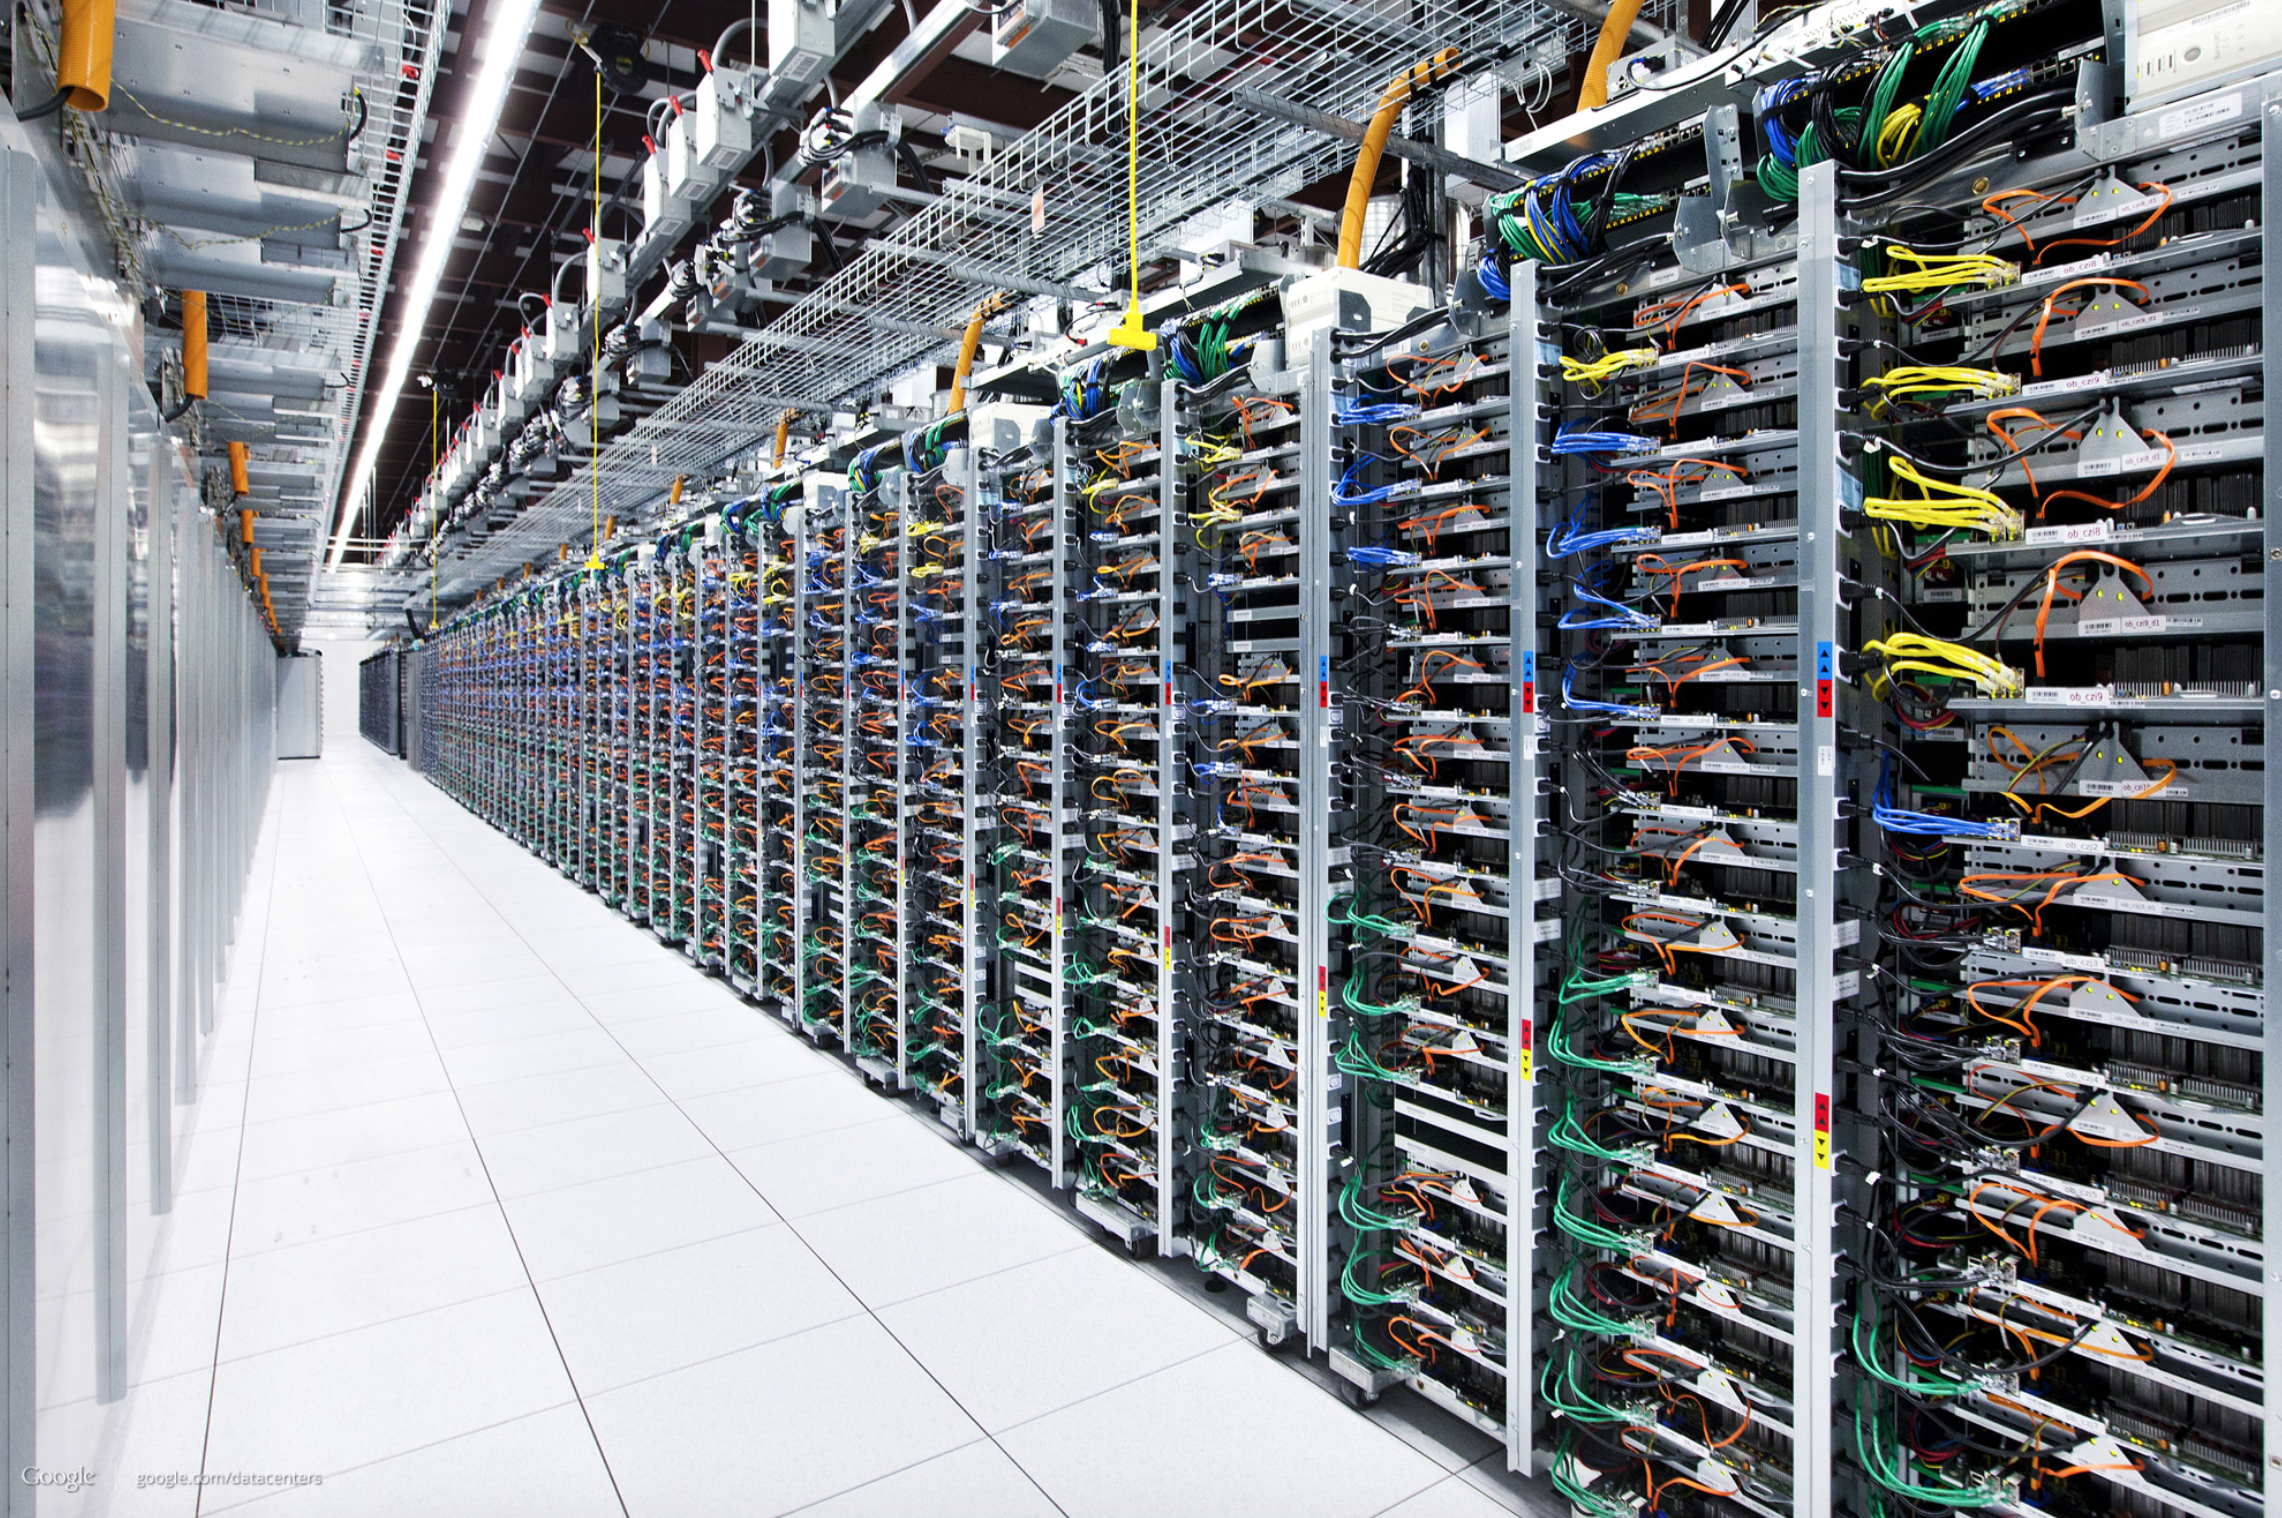
\includegraphics[width=.8\textwidth]{presentation/google_data_center}
  \end{figure}

    \note{
    \begin{itemize}
        \item The state of the current data centers nowadays, and the image represents a google deployement
        \item Very large scale deployements, with lots of networking devices
        \item Large scale Data Center Networks are hard to operate at a highly efficient and cost effective way
        \item Individually managing each network device (switches, server, ...) is a time consuming task
        \item Move to cloud based environments requires planning and research to create a scalable and simple environment
    \end{itemize}
    }
\end{frame}

\begin{frame}
\frametitle{Software-Defined Networking}

\begin{columns}
\begin{column}{0.5\textwidth}<1->
\begin{itemize}
    \item Networking services are bound to a fast changing environment, there is a need for a network design methodology that supports this
            fast evolution
    \item<1->\textbf{Software Defined Networking} is a solution that provides:
    \begin{itemize}
        \item<2->\textbf{Separation of control and data planes} 
        \item<3->\textbf{Centralization of network management functions}
    \end{itemize}
\end{itemize}
\end{column}

\begin{column}{0.5\textwidth}<4->
  \begin{figure}
      \centering
      \includegraphics[width=1\textwidth]{sdn/sdn_controller_arch}
  \end{figure}
\end{column}
\end{columns}
\end{frame}

\begin{frame}
\frametitle{Basebox}
    The SDN controller plays a central role in this architecture by connecting the network applications that connect to the Northbound interface to the networking 
        devices running on the Southbound plane.
    \only<1>{
        \begin{figure}
            \includegraphics[width=.5\textwidth]{bisdn/basebox}<1->
        \end{figure}
    }
    \only<2>{
        \begin{figure}
            \includegraphics[width=.5\textwidth]{presentation/basebox_cawr_low_level}<2->
        \end{figure}
    }

    \note{
    \begin{itemize}
        \item Esta tese foi feita em parceria com a BISDN, uma empresa alema que desenvolve controladores SDN
        \item Basebox é um controlador baseado em Linux, que integra switches e controladores SDN
        \item Configurar dispositivos com base numa API familiar graças à vasta utilização de Linux em ambientes de centros de dados
        \item Possível de correr num cenário de failover, para garantir recuperação em alturas de falhas
        \item baseboxd é um daemon que liga switches com sistemas Linux, fazendo a tradução Kernel-OpenFlow         
        \item CAWR é um controlador secundário que cria uma abstração gigante de um conjunto de switches
        \item Facilita o scale up de ambientes de rede, e gestão de múltiplos dispositivos de rede.
    \end{itemize}
    }

\end{frame}

%------------------------------------------------
\section{Monitoring SDN Switches}
%------------------------------------------------
\begin{frame}[plain]
    \centering
        \Huge{Monitoring SDN Switches}
\end{frame}

\begin{frame}{Problem - Management systems}
\begin{itemize}
    \item<1->The Basebox system lacks a system for monitoring and management of the network devices. Such a system should 
    \begin{itemize}
        \item<2-> display the topology information reported by CAWR, including the internal switch links, and the LACP discovered bond interfaces on the servers,
        \item<3-> display the port and link statistics for both switches,
        \item<4-> provide an alerting system, so that network operators can be informed of changes on the network state,
        \item<5-> provide diagnostic capabilities.
        \item<6-> allow defining Quality-of-Service policies, maintaining the traffic behaviour in the network
    \end{itemize}
\end{itemize}
\end{frame}

\begin{frame}
\frametitle{Problem - Traffic characteristics}
\begin{itemize}
    \item<1->In typical Data Center Networks, their traffic characteristics show that:
    \begin{itemize}
        \item<2->For cloud data centers, the majority of traffic is internal to each rack
        \item<3->Link utilizations are low in aggregation and edge layers
        \item<4->Despite 90\% flows are small and last hundreds of milliseconds, total traffic volume is largely dominated by the remainder, called the
            \textbf{elephant flows}
    \end{itemize}
\end{itemize}
\end{frame}


%------------------------------------------------
\section{Proposed Architecture}
%------------------------------------------------
\begin{frame}[plain]
    \centering
        \Huge{Proposed Architecture}
\end{frame}

\begin{frame}{Management System Architecture}
    \only<1>{
        \begin{figure}
            \includegraphics[width=.7\textwidth]{proposed_work/proposed_system}
        \end{figure}
    }
    \note<1>{
        \begin{itemize}
            \item A proposta de um Operations Support System tem como fim o desenvolvimento de aplicações para monitorização de rede
            \item Uma interface de gestão para os controladores, permitindo expor informação sobre topologia e estatísticas
            \item Permite a maior separação de papéis na rede, onde existem ferramentas dedicadas à gestão e monitorização
            \item Aumenta a modularidade dos components \end{itemize}
    }
\end{frame}

\begin{frame}
    \frametitle{Operations Support System}
    \begin{figure}
        \includegraphics[width=.7\textwidth]{bisdn/prp_system_low_level}
    \end{figure}

    \note{
        \begin{itemize}
            \item Modifição dos controladores para expor informação disponível nos controladores através do protocolo OpenFlow
            \item Baseados numa framework de Remote Process Call, gRPC, aproveitamos o modelo de serialização, e as definições de serviços RPC, para criar os 
                endpoints entre o OSS e os controladores
            \item Modelamos a informação de acordo com modelos de dados standardizados pela IETF
        \end{itemize}
    }
\end{frame}

\begin{frame}
\frametitle{Proof-of-concept}
    \begin{itemize}
        \item As a proof-of-concept for the Operations Support System, we have developed two systems:
        \begin{itemize}
            \item A Graphical User Interface for visualisation of the exposed information like port statistics and physical network topology;
            \item An intelligent system so that traffic changes and elephant flows can be detected.
        \end{itemize}
    \end{itemize}
\end{frame}

\begin{frame}{Proposed Algorithm}
    \begin{algorithm}[H]
        \caption{Elephant Detection Algorithm - High Level} \label{alg:high_level}
        \begin{algorithmic}[1]
            \Procedure {Elephant Flow Detection}{}
                \State Initialization
                \Loop
                    \State Query controller
                    \State Calculate the prediction error
                    \State Predict the next values
                    \State Detect the elephant flows
                    \If {Detection}
                        \State Raise Alarm
                    \EndIf
                    \State wait 2 seconds
                \EndLoop
            \EndProcedure 
           \end{algorithmic}
    \end{algorithm}

    \note{
        \begin{itemize}
            \item O algoritmo é composto por várias fases, onde:
            \item a etapa de inicialiação aprende o estado do tráfego "normal" da rede. Nesta etapa considera-se que não existem condições de tráfego anómalas
            \item o sistema de deteção de mudança de tráfego é feito com base na diferença entre o valor medido, e o valor originado pela previsão 
                anterior
            \item o cálculo das previsões é feito com base na função de exponential smoothing, onde os valores históricos determinam o valor mais um
            \item A deteção dos elephant flows é feito com base num Algoritmo de deteção, que controla os desvios face a um valor pré estabelecido
        \end{itemize}
    }
\end{frame}

%------------------------------------------------
\section{Implementation and Proof-of-concept}
%------------------------------------------------

%------------------------------------------------
\subsection{Management API}
%------------------------------------------------

\begin{frame}{Graphical User Interface}
    \begin{figure}[!tbph]
      \centering
      \includegraphics[width=0.8\textwidth]{bisdn/cawr_gui}
      \caption {CAWR topology, with the underlying switch topology}
    \end{figure}
\end{frame}

\begin{frame}{Proof-of-concept}
    \begin{figure}[!tbph]
      \centering
      \includegraphics[width=0.7\textwidth]{bisdn/basebox_gui}
      \caption {baseboxd's statistics, with the statistics of a single port}
    \end{figure}
\end{frame}

%------------------------------------------------
\subsection{Meter the Elephant}
%------------------------------------------------

\begin{frame}{Testing Environment}
    \begin{figure}
        \includegraphics[width=.7\textwidth]{meter_eleph/testing_setup}
    \end{figure}

    \note{
    \begin{itemize}
        \item Due to the differences between the OF-DPA compliant hardware switches and the standard OpenFlow implementation used in the virtualised 
            network Mininet, testing the elephant flow detection mechanism proved impossible with Basebox, which led us to choosing a different controller
        \item The controller chosen was Floodlight, due to simplicity of installation and REST interface
        \item For development of the Graphical User Interface, the standard Basebox topology was used
    \end{itemize}
    }
\end{frame}

\begin{frame}{Error calculation}
    \begin{figure}
        \includegraphics[width=1\textwidth]{meter_eleph/error_plot_sse}
        \caption{The prediction error obtained during the run time of the algorithm}
    \end{figure}

    \note{
        \begin{itemize}
            \item de forma a poder ajustar os parametros do cálculo de previsão, fazem-se análises para dois valores de $\alpha$. A tendencia ascendente
                do grafico de cima fornece piores resultados para o calculo de previsao, pelo que foi escolhido valores proximos de 1, reduzindo o impacto
                de valores anteriores
            \item Considerou-se para obter este gráfico, os erro quadrático de previsão, para diminuir o impacto de mudanças menores no tráfego nas portas.
        \end{itemize}
    }
\end{frame}

%\begin{frame}{Detection}
    %\begin{figure}
        %\includegraphics[width=.8\textwidth]{meter_eleph/detect_dumb}
        %\caption{First detection results}
    %\end{figure}
%\end{frame}

%\begin{frame}{Detection}
    %\begin{itemize}
        %\item Previous detection results are not ideal, purely comparing the output
            %of a value to a pre selected threshold, and raising several alarms
            %even no change has been detected
        %\item The CUSUM algorithm is commonly used for change detection mechanisms employed
            %in economics, health care, industrial engineering, ...
        %\item Allows for keeping track of a parameter of an output of a process, and 
            %compare it to pre selected thresholds, guaranteeing that the process is "in control"
    %\end{itemize}

    %\begin{figure}
        %\includegraphics[width=1\textwidth]{meter_eleph/offline_cusum_output}
        %\caption{Offline CUSUM output}
    %\end{figure}
%\end{frame}

\begin{frame}{Detection}
    \begin{itemize}
        \item The CUSUM algorithm is commonly used for change detection mechanisms employed
            in economics, health care, industrial engineering, ...
        \item Allows for keeping track of a parameter of an output of a process, and 
            compare it to pre selected thresholds, guaranteeing that the process is "in control"
        \item<1->Adaptation of the CUSUM algorithm to an online context is based on a sliding window
            method 
    \end{itemize}

    \begin{figure}<1->
        \includegraphics[width=.6\textwidth]{meter_eleph/detection_results_plotted}
        \caption{Online CUSUM output}
    \end{figure}

    \note{
        \begin{itemize}
            \item o algoritmo selecionado esta presente em sistemas de detecao usados em multiplos cenarios, que levanta alarmes quando se
                deteta uma mudanca;
            \item E tipicamente usado em contextos offline, onde a detecao e feita tendo em conta os dados todos
            \item A adaptacao do algoritmo CUSUM foi feita com base numa janela deslizante, para podermos nao so aplicar 
                este algoritmo de forma online, mas tambem reduzir a quantidade de dados que sao guardados para se calcular 
                a mudanca de trafego
        \end{itemize}
    }
\end{frame}

\begin{frame}{Detection}
    \begin{figure}
        \includegraphics[width=.7\textwidth]{meter_eleph/evaluation_error}
        \caption{Comparison of the number of alarms raised by the enhanced (top) and non enhanced (bottom) versions}
    \end{figure}

    \note{
        \begin{itemize}
            \item Embora o algoritmo nao seja aplicado de forma offline, podemos estabelecer um baseline de numero de alarmes,
                e o tempo de detecao esperado para a forma online, para que se veja o efeito da janela no calculo dos alarmes
            \item Neste grafico podemos ver a variacao causada quando se aplica o algoritmo cegamente. O tamanho da janela tem uma
                relacao direta com o numero de alarmes, ja que os mesmos alarmes irao ser levantados repetidamente.
            \item Tambem pode acontecer que, com uma janela grande o suficiente, os alarmes levantados ja tenham sido num tempo suficientemente
                passado, que ja nao tenham relevancia
        \end{itemize}
    }
\end{frame}

\begin{frame}{Detection}
    \begin{figure}
        \includegraphics[width=.9\textwidth]{meter_eleph/single_elephant_flow}
        \caption{Single Elephant Flow}
    \end{figure}

    \note{
        \begin{itemize}
            \item De seguida fazemos a analise de um unico elephant flow, de forma a obter uma baseline para o tempo de detecao e para o numero de
                alarmes. Estas metricas irao especificar o efeito da janela, permitindo-nos escolher qual o tamanho da janela mais adequado para cada
               utilizacao
        \end{itemize}
    }
\end{frame}

\begin{frame}{Evaluation of detection algorithm}
    \begin{figure}
        \includegraphics[width=.7\textwidth]{meter_eleph/time_error}
        \caption{Detection time difference for different window sizes}
    \end{figure}

    \note{
        \begin{itemize}
            \item Este grafico apresenta a diferenca do tempo de detecao, de acordo com o tamanho da janela.
            \item Nenhuma dos valores de janela proporciona grandes diferencas, ao contrario do resultado esperado de diminuicao do tempo
                de detecao de acordo com a diminuicao do tamanho da janela
        \end{itemize}
    }
\end{frame}

\begin{frame}{Evaluation of detection algorithm}
    \begin{table}[]
        \centering
        \caption{False alarms statistics}
        \label{tab:false_alarms}
        \begin{tabular}{|c|c|c|c|c|c|}
            \hline
            Window Size   & 5        & 10       & 15  & 20  & 25  \\ \hline
            count         & 30       & 30       & 30  & 30  & 30  \\ \hline
            $\bar{x}$     & 2.833333 & 2.166667 & 2.0 & 2.0 & 2.0 \\ \hline
            $\sigma^2$    & 0.791478 & 0.379049 & 0.0 & 0.0 & 0.0 \\ \hline
        \end{tabular}
    \end{table}

    \note{
        \begin{itemize}
            \item Esta tabela permite-nos verificar o efeito do tamanho da janela com base no numero de alarmes acionados.
        \end{itemize}
    }
\end{frame}
%------------------------------------------------
\section{Conclusions}
%------------------------------------------------
\begin{frame}[plain]
    \centering
        \Huge{Proposed Architecture}
\end{frame}


\begin{frame}{Summary of Achievements}
    \item We have proposed and implemented a system that
    \begin{itemize}
        \item integrates a Software-Defined Controller environment, and exposes internal
            management information
        \item allows the development of management applications, that we have proven 
            by developing a Proof-of-Concept containing on a Graphical User Interface
        \item extends the controllers capability for monitoring network traffic, 
            by analysing traffic statistics for elephant flow detection
    \end{itemize}
\end{frame}

\subsection{Future Work}

\begin{frame}{Future Work}
    \begin{itemize}
        \item Extend the GUI for displaying VLANs and layer 3 information like routes and neighbours;
        \item Extend the traffic change monitoring for closer insights on possible offending flows;
        \item Research the capacity that the controllers have for implementation of OpenFlow meters,
            allowing us to shape individual traffic flows.
    \end{itemize}
\end{frame}

\begin{frame}{Achievements}
    \begin{figure}
        \includegraphics[width=.9\textwidth]{presentation/basebox_paris}
        \caption{Image of the developed GUI, present in the SENDATE Mid Term Event in Paris}
    \end{figure}
\end{frame}

\begin{frame}[plain]
\centering
    \Huge{{Thank your for you attention!}}
\end{frame}

\end{document}
              
